The next defensive structure we introduce is partially in response to the claim in
\cite{goodfellow2015explaining} about dot products wildly changing as a result of how many
components are multiplied within it. Further, it is ``inspired'' (in the loosest sense,
authoritatively speaking) by this author's very unscientific and personal experience when trying to
decipher hard-to-understand objects, visually speaking.

Let's say that we have a group of pixels for which we need to decipher what it represents. In this
case, the group takes on some kind of noise which makes it hard to recognize, yet the general themes
are still contained within the group (for example, it might be a very dark patch that needs careful
examinations of the relationship between connected components within it). Personally, the author
tries to find these connected components and perform the comparison. So, with that in mind, we
extend this technique to the deep learning case.

Inspired by convolutional neural networks, we take adjacent patches of pixels, and, in order to
approximate the connected-components analogy, we simply compare each pixel (or in the three-channel
case, subpixel, which we will refer to from here on) to every other within the patch. The way we
chose to compare subpixels is via a modification of the Distance Matrix\cite{wikipediadm}. Instead
of squaring the difference between subpixel values, we do not square at all. The reason for this is
simple: in the standard image processing case, distance would result in the same output when one
subpixel is less than or greater than the other used in the comparison. For this use case, that is
not necessarily ideal: if one pair is the inverted version of another within the image, they would
get the same distance value, but the inversion should really be considered a different relationship.

In mathematical terms, what follows is the definition of the difference matrix, $D$. Each subpixel
at position $j$ in the vector $\mathbf{v}$ that holds every element in the patch is subtracted from
element $i$ from that same vector. This creates the element $D_{ij}$; in other words, the index of
the subpixel from which element $j$ is being subtracted is $i$. Again, notice that this is derived
from the definition of the distance matrix, except in that case, $D_{ij}$ is actually $\left(
\mathbf{v}_i - \mathbf{v}_j \right)^2$. See figure \ref{pairwisedepiction} for a graphical view of
this neuron's layout.

\begin{figure}
    \begin{center}
        \begin{tabular}{c c c}
            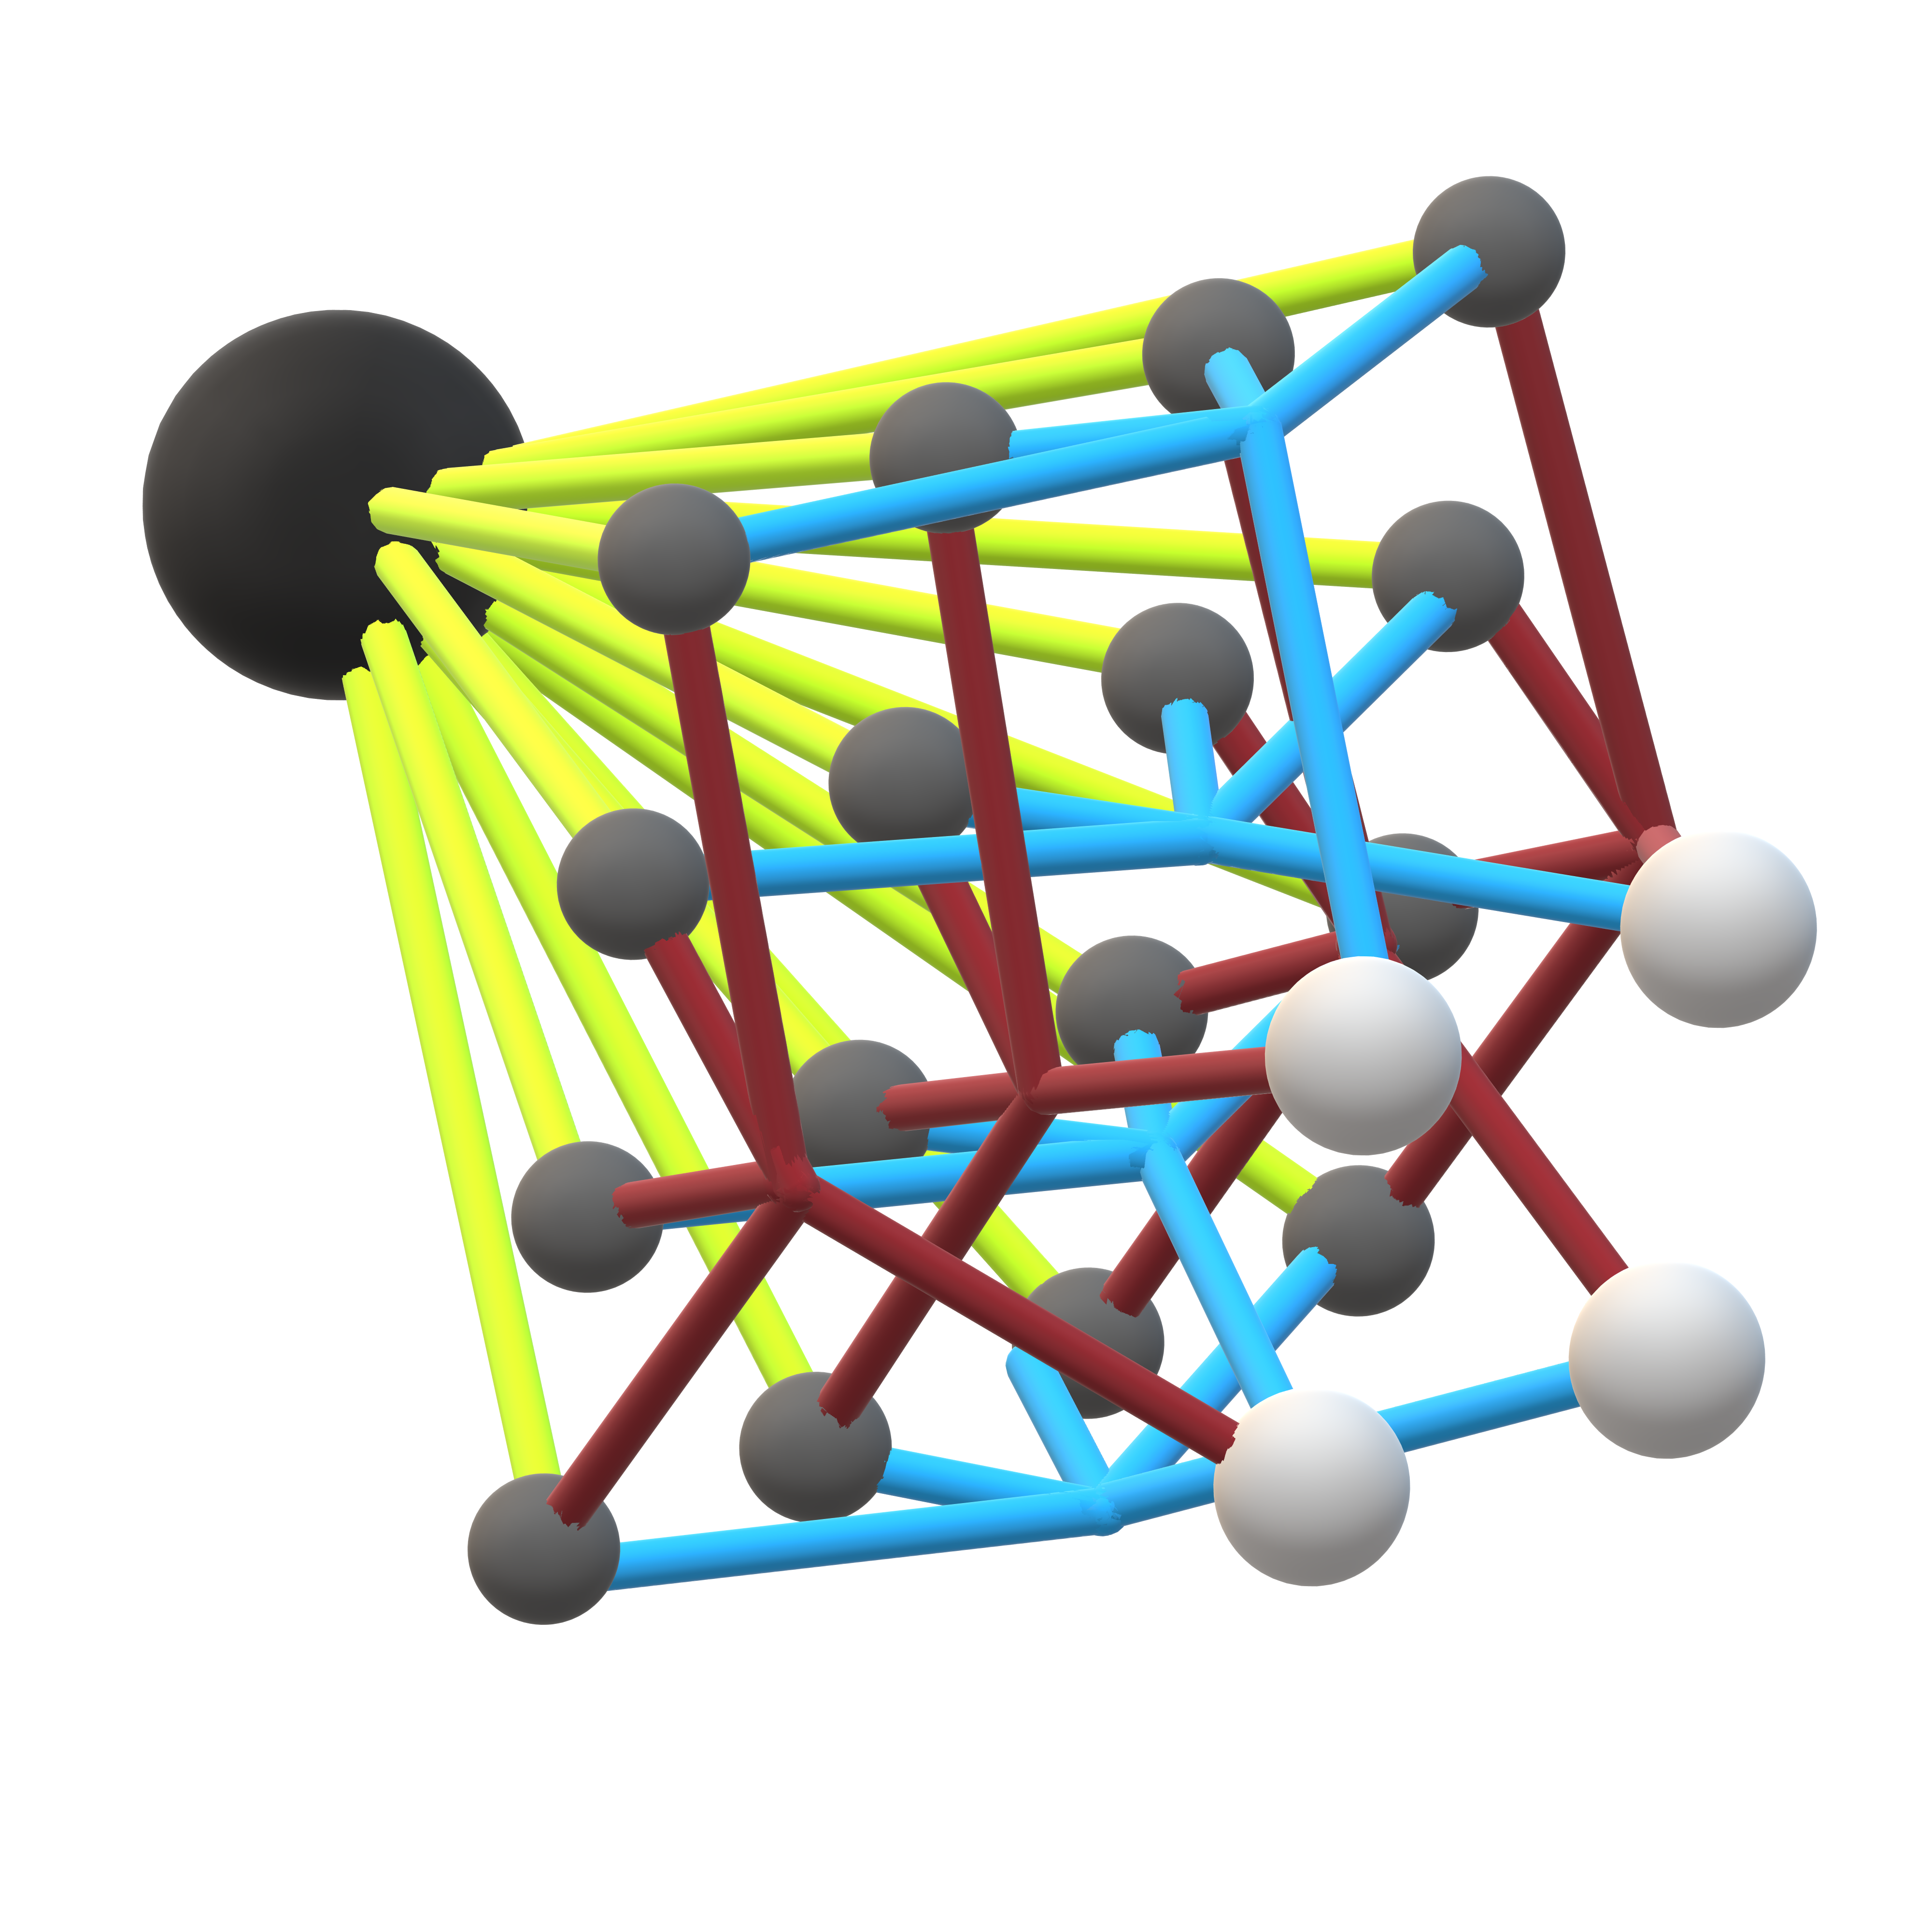
\includegraphics[width = 2in]{Friendly/LaTeX/figures/pairwiseview1.png} & 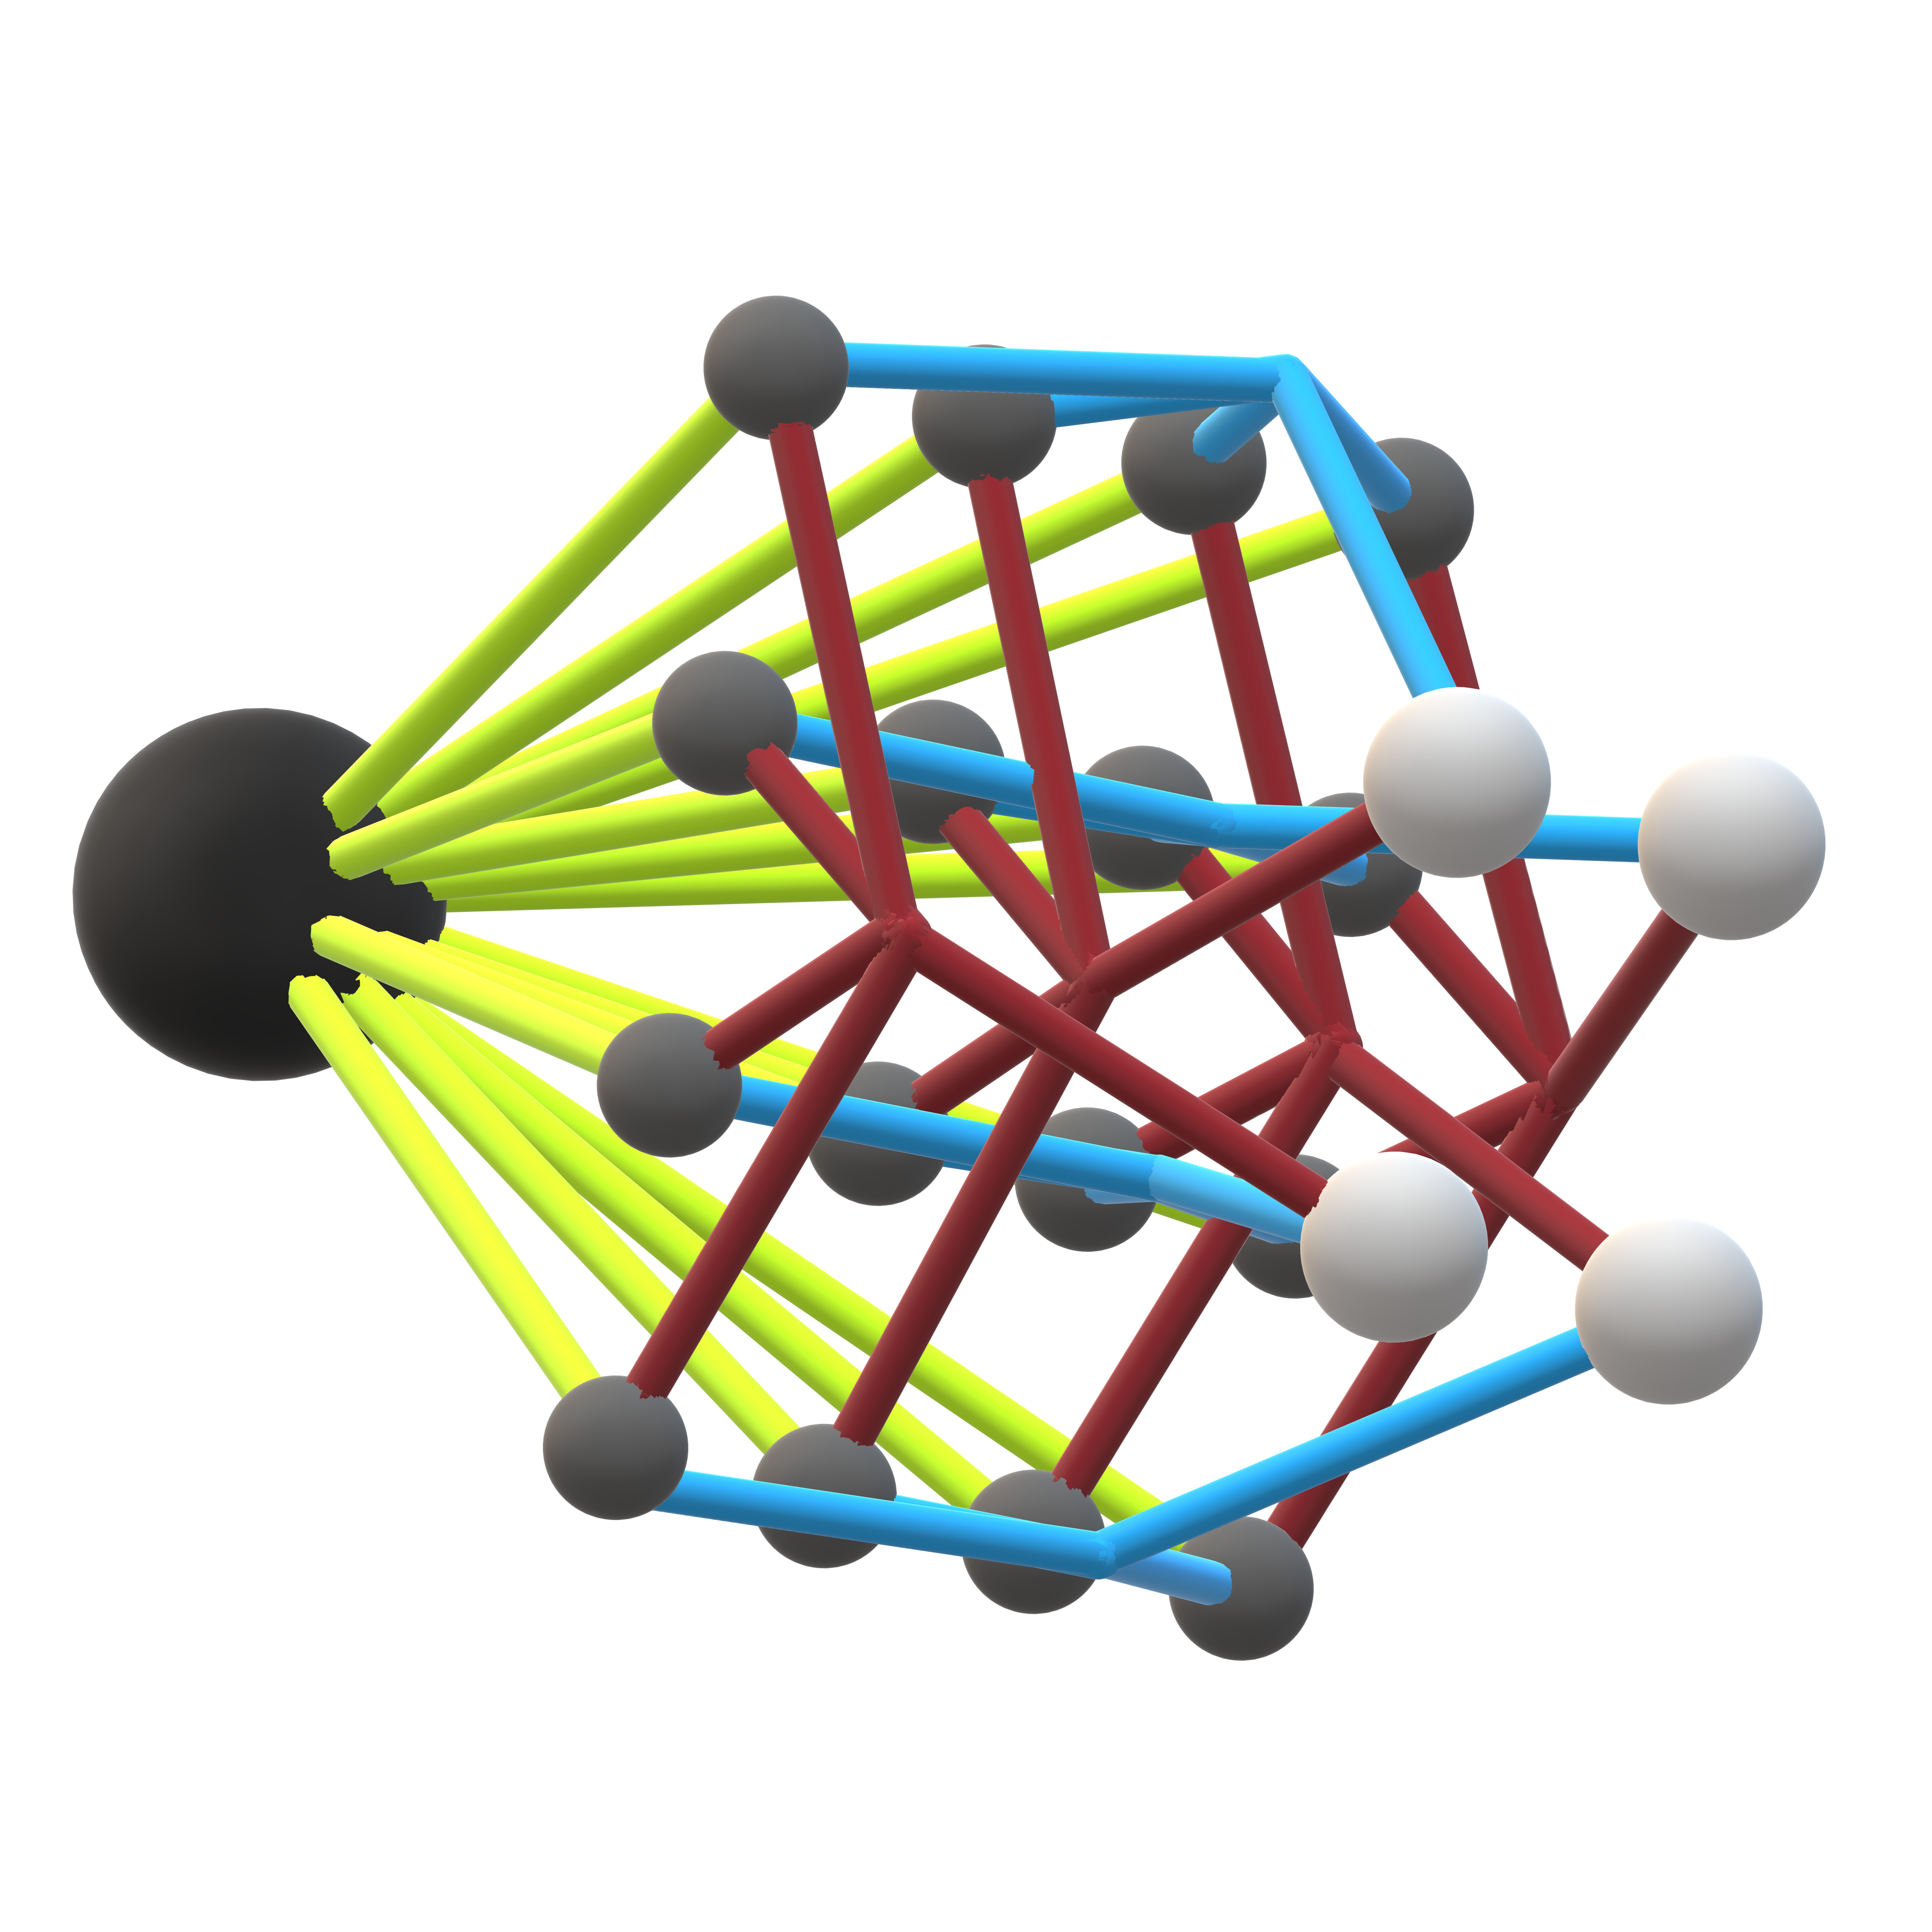
\includegraphics[width = 2in]{Friendly/LaTeX/figures/pairwiseview2.png} & 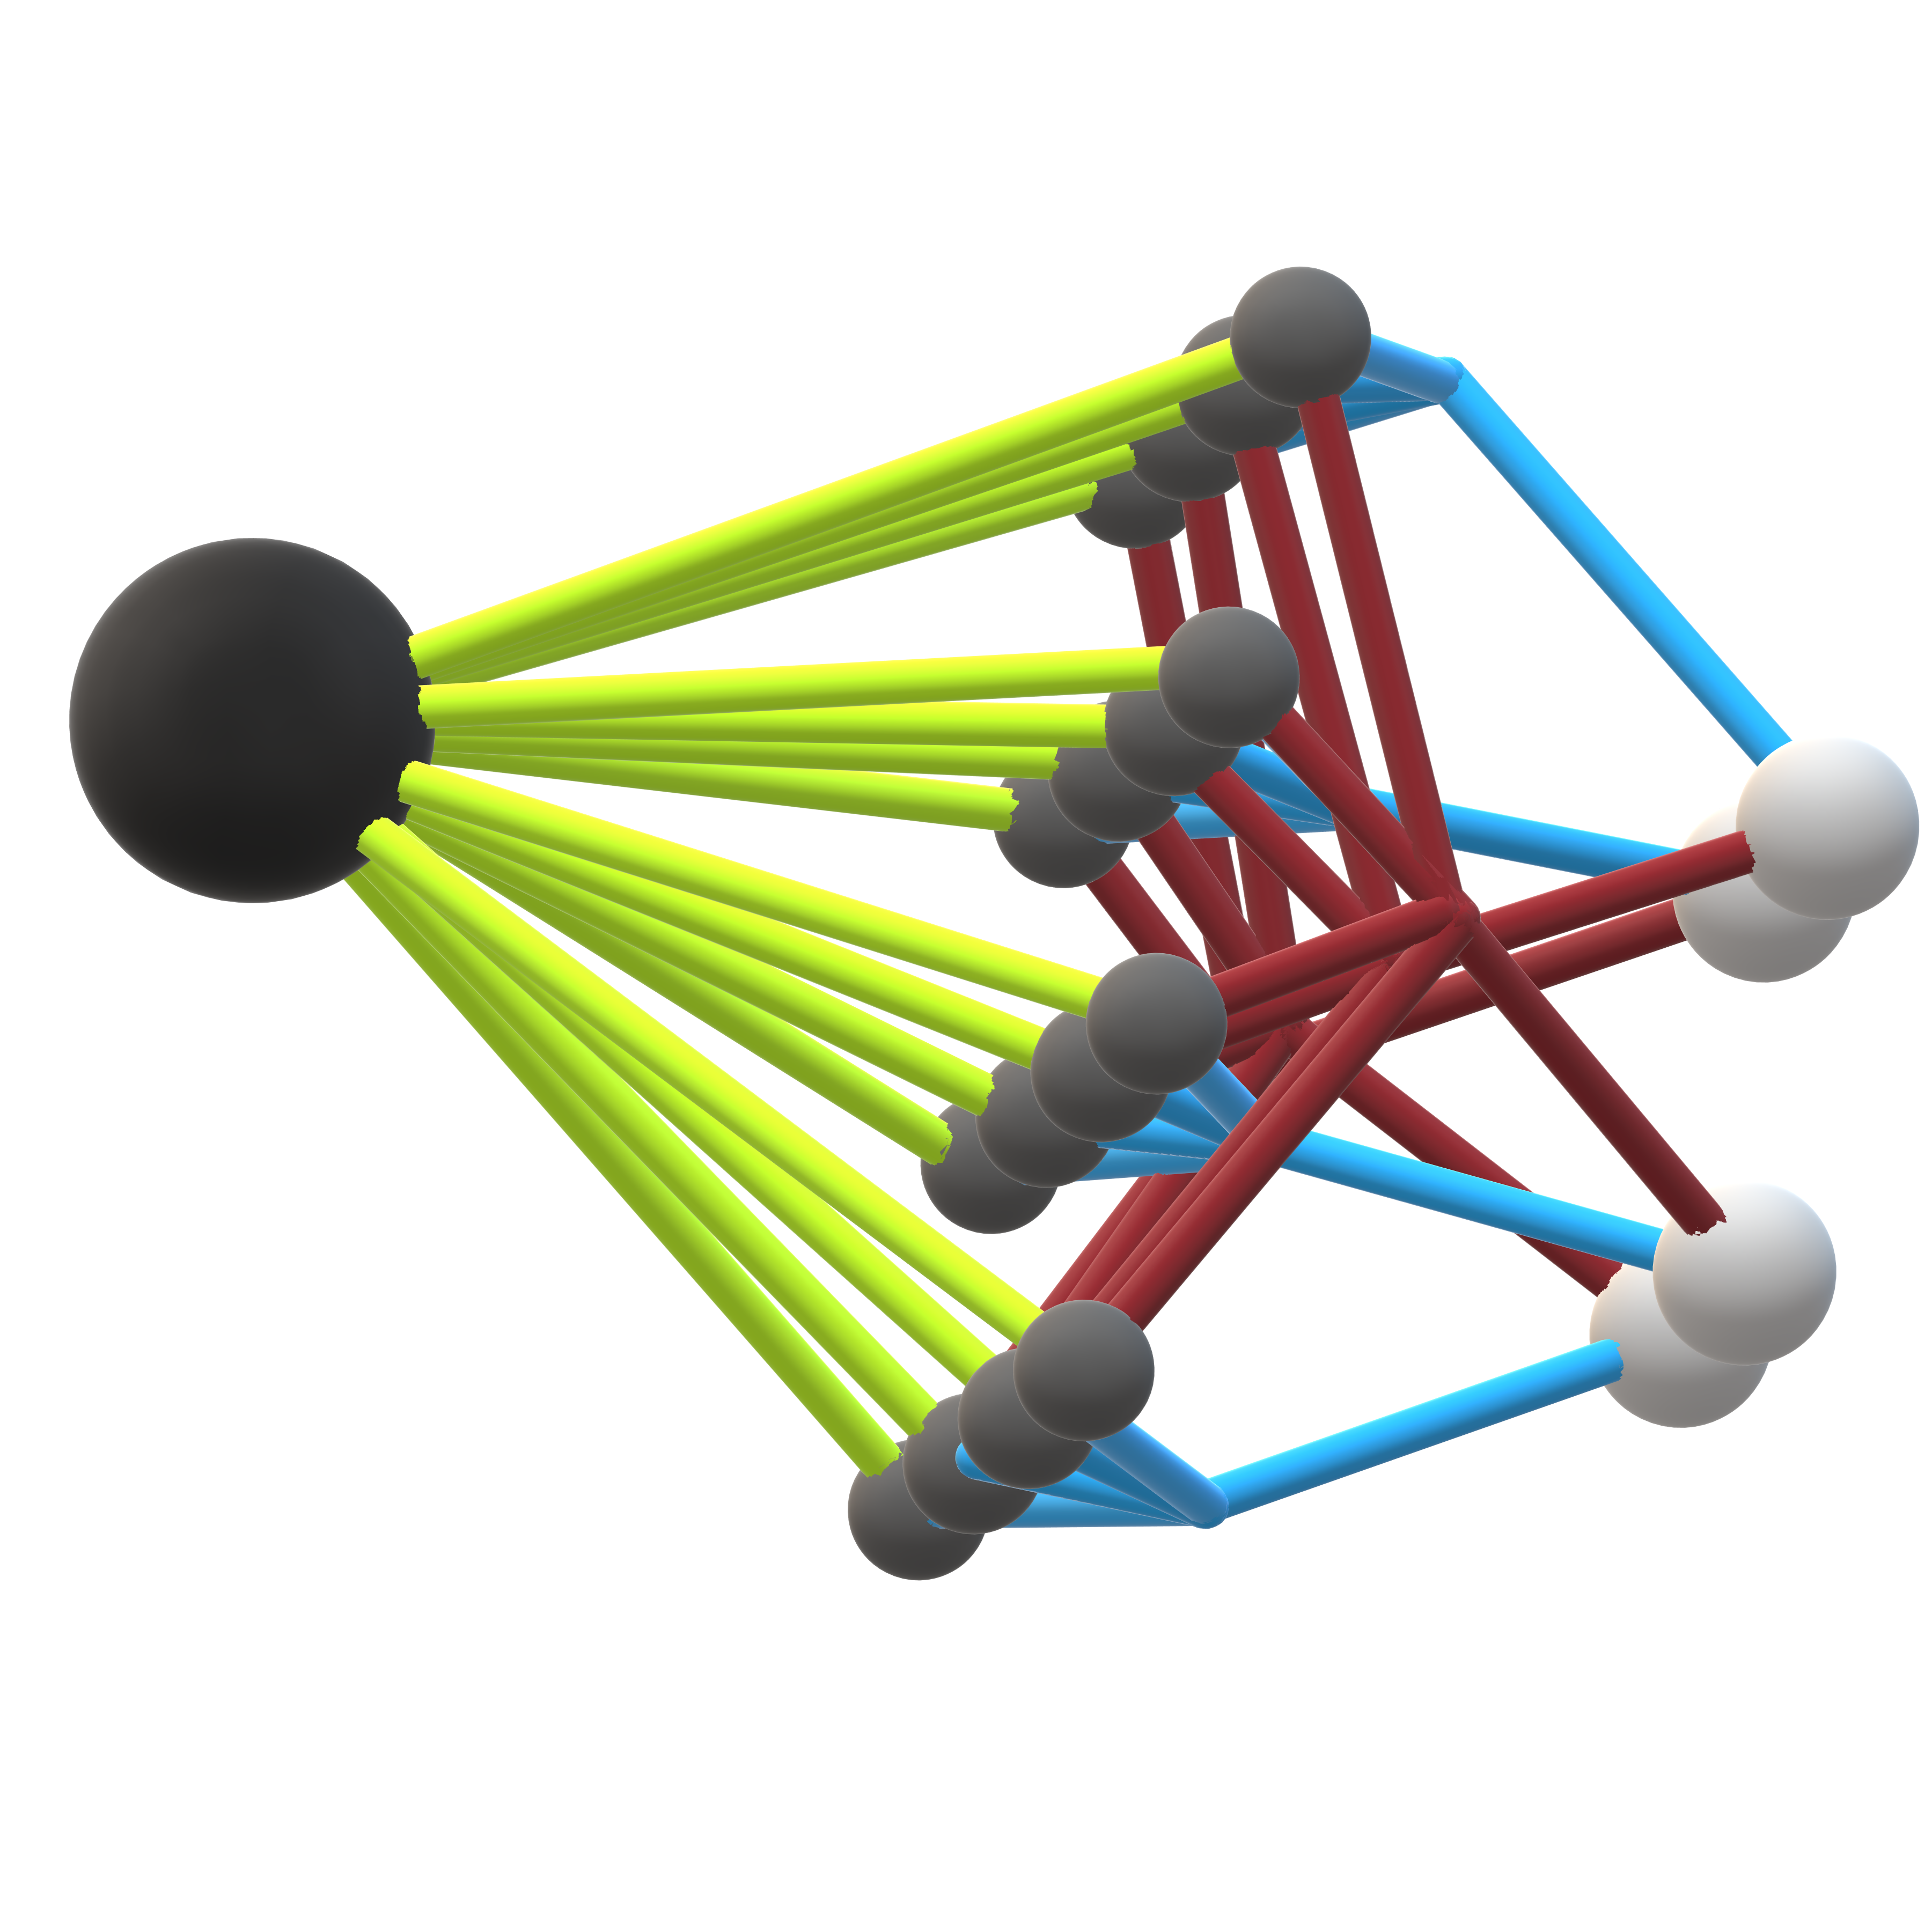
\includegraphics[width = 2in]{Friendly/LaTeX/figures/pairwiseview3.png}
        \end{tabular}
    \end{center}
    \caption{Visual of Pairwise Difference. From light to dark, the spheres represent the input, the
             subtaction + sigmoid, and the output of pairwise difference (sans the activation
             function). Burgundy lines indicate that the value it links from is being subtracted
             from the teal line's equivalent. Generated using Paint 3D~\cite{msftprogram}.}
    \label{pairwisedepiction}
\end{figure}

The difference matrix alone does not actually solve the problem described in
\cite{goodfellow2015explaining}; this is because, if all these subtractions are used in a neuron by
multiplying each subtraction by one of the neuron's weights, noise added to a patch causes noise in
the subtractions, which leaves us at the same issue (or possibly even worse given the squared number
of elements, although we have not done the math to prove this claim). Further, we just want to know
how the subpixels compare, not how they subtract. As a result, before the dot product of the neuron,
we put each subtraction through a sigmoid activation function. At the first layer, if the input
contains integer values (as is the common representation of subpixels), we won't see much change in
the sigmoid in the face of noise as the range of values is typically 0 to 255, whereas the sigmoid
activation function plateaus not far (relatively speaking) from the origin. This is the benefit of
pairwise comparisons: small changes in a subpixel values do not have the same effect on the
comparison (just between two subpixels) as it does on a dot product. To wrap up, the output neuron
does not require any specific activation function, as most of the flatness comes from the preceding
sigmoid functions. We call this neuron \textit{Pairwise Difference}.

However, there is still a rather large elephant in the room: computational complexity is essentially
squared, as we are building a pairwise matrix from a single vector. This is not a trivial problem to
address; for example, one might just use the non-zero values in the upper triangle of $D$ because
$D$ is antisymmetric, so the information gain of keeping the lower triangle is (hopefully) very minimal, at
least for $D$. However, this method suffers from not being able to treat the non-commutativity of
subtraction differently, as there is no weight for the second permutation of the operands of
subtraction. Further, effectively halving the number of inputs to the dot product only reduces the
dot product complexity by a constant factor, so, theoretically, larger and larger kernels, from a
practical standpoint, still might be out-of-reach. An alternative to the difference matrix might be
that, as in the ``mini-networks'' of Inceptionv3\cite{szegedy2015rethinking}, we do tiny dot
products, and then take dot products of those tiny dot products, etc. Each tiny dot product would
need to go through an activation (a pseudo-mimic of the difference matrix with just a few elements
participating in the dot product) as, otherwise, the result of the ``mini-network'' would be very
similar to a normal dot product from the perspective of \cite{goodfellow2015explaining}. A third
method would be to use this type of layer on just the image as most of the noise filtering will
likely occur within that layer.

In addition to these computational issues, when programming such layers, it is very easy for memory
complexity to grow as quickly as computational complexity. This is due to the fact that, in
frameworks such as Chainer\cite{tokui2019chainer} and PyTorch\cite{NEURIPS2019_9015}, at the very
least, it is easy to inadvertently suffer from holding the full difference matrix in memory. We can
get around this by performing the subtraction, sigmoid, and weight multiplication operations
one-at-a-time for each pair formed by a reference subpixel $p_i$ with static index $i$ and every
other subpixel $p_j$ in the kernel; if this happens for each static subpixel, we end up with a dot
product for every reference pixel, which requires a single value of appropriate size in memory.
Parallelization can still occur by doing this for each $i$ simultaneously. Note that this does not
differ from the memory requirements of holding each subpixel in memory, which is a tractable usage
of memory. However, at the time of writing, this implementation had not been finished.

From a gradient standpoint, Pairwise Difference is a little complicated. Following the intuition
of \cite{IMM2012-03274}[eqns. 136] where every path a gradient can take to a variable has a gradient
that must by multiplied by the gradient from the start of the path to the variable (this is used in the multivariable
chain rule, whose necessity was made clear to us by \cite{li}[``Gradients add up at forks'']), there are two
types of paths for our specific problem where this may be the case:
\begin{enumerate}
    \item the paths attributable to each image in the batch, and
    \item the paths inside those paths that are associated with each spot to which the neuron was
          applied
\end{enumerate}
Note that these are really just the same paths (all these paths fit case 2), but they are separated
here to show that there is a hierarchy of paths, which may ease the understanding of the following
derivation of Pariwise Distance's derivative.

For one patch $p$ of one sample in the batch (that has been processed by layer $i$'s neuron, $n_i$,
contained in a Pairwise Difference layer), the output of $n_i(p)$ is a dot product between the
sigmoid-filtered subtractions between each element $r$ and element $s$ in the patch and $n_i$'s
weights, $w_{rs}$. We will call ``$\text{sig}$'' the sigmoid activation function and
``$\text{sub}$'' subtraction formulated as $\text{operand}_1 - \text{operand}_2$. The derivative
with respect to $w_{rs}$ is
\[
    \frac{\partial n_i}{\partial w_{rs}}
    = \frac{\partial}{\partial w_{rs}}  \sum_{a \in p} \sum_{b \in p} w_{ab} \cdot \text{sig}(\text{sub}(a, b))
    = \frac{\partial}{\partial w_{rs}}  w_{rs} \cdot \text{sig}(\text{sub}(a, b))
    = \text{sig}(\text{sub}(a, b))
\]
Each of the volumes (one for each sample in the batch) uses $w_{rs}$ (abstracting away $p$ so that
it represents just the patch that would be taken out at $p$'s location). According to the multivariable
chain rule, for a loss function $L$, $\frac{\partial L}{\partial w_{rs}}$ is the summation of the
partial derivatives calculated by multiplying $\frac{\partial L}{\partial n_i}$ by
$\frac{\partial n_i}{\partial w_{rs}}$.

To keep backpropagation\cite{rumelhart} going to the previous layer, we also need to know
$\frac{\partial n_i}{\partial r}$ (where, again, $r$ is in $p$). In a fashion similar to $w_i$,
$r$ participates indirectly in multiple dot products against many different weights. Not only is $r$
used in $\text{sig}(\text{sub}(r, r'))$ where $r'$ is any element in $p$, but it is used in the other direction,
$\text{sig}(\text{sub}(r', r))$. For the former, the derivative for each of these is
\[
    \frac{\partial \text{sig}}{\partial \text{sub}(r, r')} \frac{\partial \text{sub}(r, r')}{\partial r}
    = \frac{\partial \text{sig}}{\partial \text{sub}(r, r')} (1)
    = \frac{\partial \text{sig}}{\partial \text{sub}(r, r')}
\]
and for the latter, it is
\[
    \frac{\partial \text{sig}}{\partial \text{sub}(r', r)} \frac{\partial \text{sub}(r', r)}{\partial r}
    = \frac{\partial \text{sig}}{\partial \text{sub}(r', r)} (-1)
    = - \frac{\partial \text{sig}}{\partial \text{sub}(r', r)}
\]
Again, since the multivariable chain rule allows us to add all pairs of these derivatives together,
for all patches $P_r$ that contain $r$, we end up with the derivative being
\begin{multline}
    \sum_{p \in P_r} \sum_{n \in neurons} \frac{\partial n}{\partial r}
    = \sum_{p \in P_r} \sum_{n \in neurons} \sum_{r' \in p} \left[ \frac{\partial n(p)}{\partial \text{sub}(r, r')} \frac{\partial \text{sub}(r, r')}{\partial r} + \frac{\partial n(p)}{\partial \text{sub}(r', r)} \frac{\partial \text{sub}(r', r)}{\partial r} \right]\\[10pt]
    = \sum_{p \in P_r} \sum_{n \in neurons} \sum_{r' \in p} \left[ \frac{\partial n(p)}{\partial \text{sub}(r, r')} (1) + \frac{\partial n(p)}{\partial \text{sub}(r', r)} (-1) \right]\\[10pt]
    = \sum_{p \in P_r} \sum_{n \in neurons} \sum_{r' \in p} \left[ \frac{\partial n(p)}{\partial \text{sub}(r, r')} - \frac{\partial n(p)}{\partial \text{sub}(r', r)} \right]
\end{multline}
The derivatives that remain in this equation are easy to derive based on the description of Pairwise
Difference (a simple multivariable chain rule application), so we do not find it necessary to do so
here.







